%
% teil2.tex -- Beispiel-File für teil2 
%
% (c) 2020 Prof Dr Andreas Müller, Hochschule Rapperswil
%
% !TEX root = ../../buch.tex
% !TEX encoding = UTF-8
%
\section{Kreisspiegelung\label{geradlinig:section:kreisspiegelung}}
\kopfrechts{Kreisspiegelung}
Die Kreisspiegelung ist eine Transformation der ebenen Geometrie, 
welche das Innere und Äussere eines Kreises vertauscht.
Diese Transformation ist winkeltreu.
Für einen Kreis mit Mittelpunkt $M$ und Radius $R$ wird der Bildpunkt $P'$ 
eines Punktes $P$ dadurch definiert, 
dass $P'$ auf der Geraden $MP$ liegt und die Bedingung
\begin{align}
    \overline{MP'}\cdot\overline{MP} = R^2
    \label{eq:constant0}
\end{align}
erfüllt.
Wird anstelle eines einzelnen Punktes eine Gerade gespiegelt, 
entsteht wieder ein Kreis, 
welcher durch den Mittelpunkt $M$ des Inversionskreises verläuft.
Dies ist in Abbildung~\ref{fig:kreisspiegelung} dargestellt.
Die Punkte der ursprünglichen Geraden, welche sich im Unendlichen befinden, 
werden dabei auf den Mittelpunkt $M$ abgebildet.
\begin{figure}
    \centering
    \begin{minipage}{0.49\textwidth}
        \centering
        \raisebox{0.1\height}{%
            \begin{tikzpicture}[scale=2]

  % Circle center M and radius R
  \coordinate (M) at (0,0);
  \def\R{0.8}

  % Point P and R
  \coordinate (P) at (1.2,0.8);
  \coordinate (R) at ({\R*cos(60)},{\R*sin(60)});

  % Inversion factor
  \pgfmathsetmacro{\k}{0.25}

  % Inverted point P'
  \coordinate (Pp) at (\k*1.2, \k*0.8); % same coordinates as P

  % Circle
  \draw[darkgreen, line width=1.8pt] (M) circle (\R);

  % Line through M, P', P
  \draw[black, thick] (M) -- (Pp) -- (P);
  \draw[black, thin] (M) -- (R);

  % Points
  \fill[blue] (P) circle (1pt);
  \fill[red] (Pp) circle (1pt);
  \fill[black] (M) circle (1pt);

  % Labels
  \node[left] at (M) {$M$};
  \node[below] at (P) {$P$};
  \node[below] at (Pp) {$P'$};
  \node[above right, yshift=-1pt, xshift=-1pt] at (R) {$R$};

\end{tikzpicture}
%
        }
    \end{minipage}
    \hfill
    \begin{minipage}{0.49\textwidth}
        \centering
        \begin{tikzpicture}[scale=2]

  % Circle center M and radius R
  \coordinate (M) at (0,0);
  \def\R{0.8}
  \def\r{0.3}

  % Circles and Line
  \draw[darkgreen, line width=1.8pt] (M) circle (\R);
  \draw[red, line width=1pt] ($(M)+(\r,0)$) circle (\r);
  \draw[blue, thick] ($(M)+(1.2,-1.2)$) -- ($(M)+(1.2,1.2)$);
  \draw[blue, thin, dashed] ($(M)+(1.2,-1.4)$) -- ($(M)+(1.2,1.4)$);

  % Points
  \fill[black] (M) circle (1pt);
  \fill[red] ({2*\r},0) circle (1pt) node[black, left] {$P'$};
  \fill[blue] (1.2,0) circle (1pt) node[black, right] {$P$};

  % Labels
  \node[left] at (M) {$M$};

\end{tikzpicture}

    \end{minipage}
    \caption{Illustration der Kreisspiegelung~\cite{kreisspiegelung} links
    mit einem roten Punkt $P'$ der in den blauen Punkt $P$ abgebildet wird. 
    Rechts ein Beispiel an einem roten Kreis, welcher in eine blaue Gerade abgebildet wird.
    Der grüne Kreis ist der sogenannte Inversionskreis dieser Transformation.}
    \label{fig:kreisspiegelung}
\end{figure}

\subsection{Peaucellier-Lipkin-Mechanismus}
Die Eigenschaft der Kreisspiegelung, einen Kreis auf eine Gerade abzubilden,
wird beim Peaucellier-Lipkin-Mechanismus verwendet.
Die geometrische Darstellung dieses Mechanismus besteht aus sechs Stäben, 
wie in Abbildung~\ref{fig:geometrie_peauc} dargestellt.
Die Längen $\overline{OA}$ und $\overline{OC}$ sind gleich gross.
Die vier Stäbe $AB$, $BC$, $CD$ und $DA$ 
besitzen ebenfalls dieselbe Länge und bilden dadurch einen Rhombus.
Der Punkt $O$ ist dabei fest im Raum verankert.

Wird der Punkt $B$ auf einer Kreisbahn geführt, 
welche durch den Punkt $O$ verläuft, 
bewegt sich der Punkt $D$ zwingend entlang einer Geraden.
Dies kann beispielsweise durch einen zusätzlichen Stab erreicht werden, 
deren Länge der Hälfte von $\overline{OB}$ entspricht.
Die Kreisbahn von $B$ ist in Rot dargestellt.
Im Gegensatz dazu würde sich Punkt $D$ auf einer Kreisbahn bewegen, 
wenn Punkt $B$ entlang einer Geraden geführt würde, 
welche nicht durch $O$ verläuft.
Auch dieser Kreis würde durch den Punkt $O$ verlaufen.

Es existieren viele verschiedene Proportionen dieses Mechanismus.
Die entscheidende Eigenschaft besteht darin, dass die Punkte $O$, 
$B$ und $D$ während der gesamten Bewegung kollinear bleiben.
Unter dieser Bedingung müssen lediglich die Beziehungen
$\overline{AB} = \overline{AD}$ sowie $\overline{BC} = \overline{DC}$
erfüllt sein.
Zusätzlich muss Punkt $B$ auf einer Kreisbahn geführt werden, 
welche den Punkt $O$ trifft.
Eine feste Beziehung zwischen den Längen der Seiten des Vierecks $ABCD$ 
ist nicht erforderlich.
\begin{figure}
    \centering
    \begin{tikzpicture}[scale=1.6]

  % Circle 
  \def\r{1}
  \draw[red, thick] (0,0) circle (\r);

  % Points on/around circle
  \coordinate (O) at (-\r,0);
  \coordinate (A) at (1.5,1.2);
  \coordinate (C) at (1.5,-1.2);
  
  % Vertical line
  \coordinate (B) at (\r,0);
  \coordinate (D) at (2,0); % 2 = {2*(A.x) - (B.x)}
  \coordinate (P) at ($(B)!0.5!(D)$);
  \draw[blue, thick] (2,-2) -- (2,2);

  % Connections
  \draw[thick] (O) -- (A) -- (B) -- (C) -- cycle;
  \draw[thick] (A) -- (D) -- (C);

  % Additional lines for math. proof
  \draw[darkgreen, thin, dashed] (O) -- (B) node[pos=0.5, above, yshift=-0.05cm] {$y$};
  \draw[darkgreen, thin, dashed] (B) -- (P) node[pos=0.5, above, yshift=-0.05cm] {$x$};
  \draw[darkgreen, thin, dashed] (D) -- (P) node[pos=0.5, above, yshift=-0.05cm] {$x$};
  \draw[darkgreen, thin, dashed] (P) -- (A) node[pos=0.5, right, xshift=-0.05cm] {$h$};

  % Mark points
  \fill[black] (O) circle (1.5pt) node[left] {$O$};
  \fill[black] (A) circle (1.5pt) node[above] {$A$};
  \fill[black] (B) circle (1.5pt) node[left] {$B$};
  \fill[black] (C) circle (1.5pt) node[below] {$C$};
  \fill[black] (D) circle (1.5pt) node[right] {$D$};
  \fill[darkgreen] (P) circle (1.5pt) node[below] {$P$};

\end{tikzpicture}

    \caption{Kreisspiegelung am Peaucellier-Lipkin-Mechanismus~\cite{peauc_lip_linkage}.}
    \label{fig:geometrie_peauc}
\end{figure}

\begin{satz}
    Der Peaucellier-Lipkin-Mechanismus hat die Eigenschaft
    \begin{align}
        \overline{OB}\cdot\overline{OD} = R^2
        \label{eq:constant1}
    \end{align}
    einer Kreisspiegelung.
\end{satz}
\begin{proof}
    Um diese Eigenschaft herzuleiten, ergänzen wir in
    Abbildung~\ref{fig:geometrie_peauc} den Punkt $P$.
    Dieser liegt jeweils in der Mitte der Strecken $AC$ und $BD$.
    Weiter definieren wir $\overline{OB}=y$, $\overline{PD}=x$ und
    $\overline{PA}=h$.
    Da $P$ die Mitte von $BD$ ist, gilt
    $\overline{OD}=y+2x$.
    Damit erhalten wir die neue Gleichung
    \begin{align*}
        \overline{OB}\cdot\overline{OD} 
        = 
        y(y+2x)
        =
        y^2+2xy.
    \end{align*}
    Da das Dreieck $OPA$ rechtwinklig ist, gilt nach dem Satz des Pythagoras
    \begin{align}
        \overline{OA}^2
        =
        (y+x)^2+h^2
        =
        y^2+2xy+x^2+h^2.
        \label{eq:OA}
    \end{align}
    Für das ebenfalls rechtwinklige Dreieck $PDA$ gilt
    \begin{align}
        \overline{AD}^2
        =
        x^2+h^2.
        \label{eq:AD}
    \end{align}
    Subtrahiert man Gleichung~\eqref{eq:AD} von Gleichung~\eqref{eq:OA}, erhält man
    \begin{align*}
        \overline{OA}^2-\overline{AD}^2
        =
        y^2+2xy
        =
        \overline{OB}\cdot\overline{OD}.
    \end{align*}
    Da die Längen $\overline{OA}$ und $\overline{AD}$ konstant sind, ist auch
    $\overline{OA}^2-\overline{AD}^2$ konstant.
    Folglich ist auch das Produkt
    $\overline{OB}\cdot\overline{OD}$ konstant.
    Nun stellt sich eben heraus, dass diese Konstante immer $R^2$ ist,
    wie in Gleichung~\eqref{eq:constant1}.
    Dabei ist $R$ der Radius des Inversionskreises, welcher in 
    Abbildung~\ref{fig:kreisspiegelung} grün gezeichnet ist.
\end{proof}

\subsection{Perrolatz-Mechanismus}
Ein weiterer durch die Kreisspiegelung inspirierter Mechanismus 
ist der Mechanismus von Perrolatz, 
welcher in Abbildung~\ref{fig:perrolatz_link} dargestellt ist.
Dieser besteht ebenfalls aus sechs Stäben.
\begin{figure}
    \centering
    \begin{minipage}{0.32\textwidth}
        \centering
        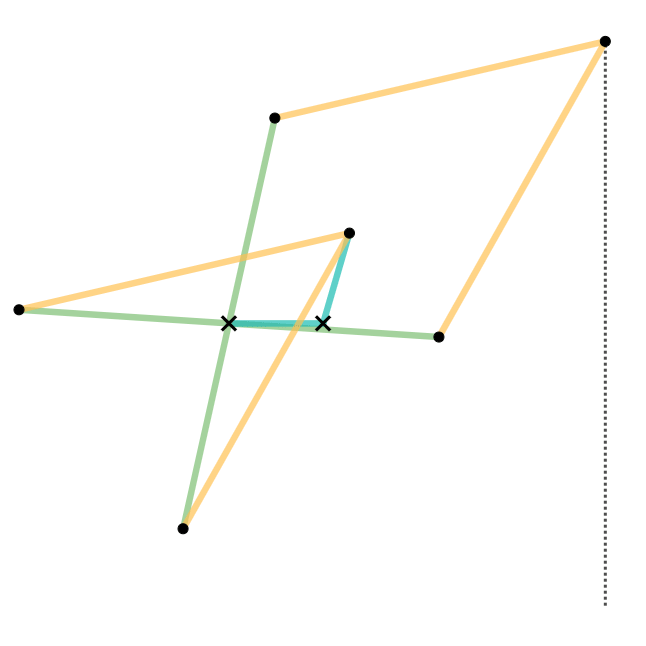
\includegraphics[width=\textwidth]{papers/geradlinig/figures/perrolatz_linkage1.png}
    \end{minipage}
    \hfill
    \begin{minipage}{0.32\textwidth}
        \centering
        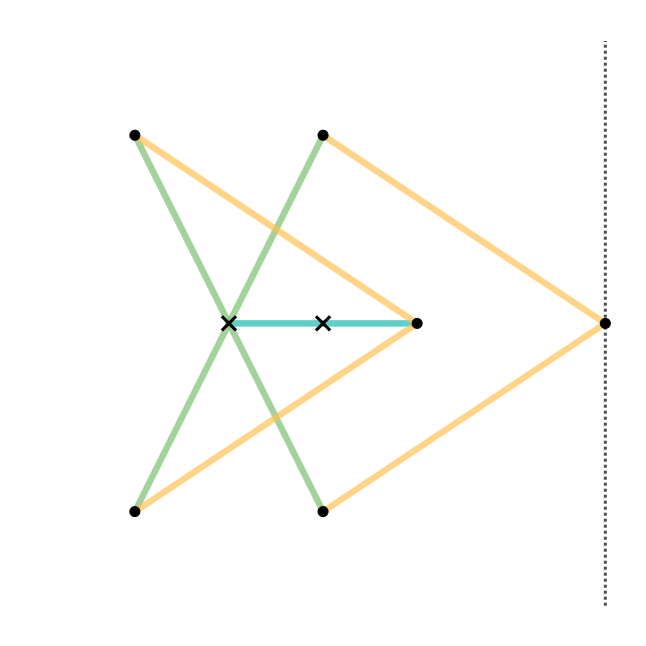
\includegraphics[width=\textwidth]{papers/geradlinig/figures/perrolatz_linkage2.png}
    \end{minipage}
    \hfill
    \begin{minipage}{0.32\textwidth}
        \centering
        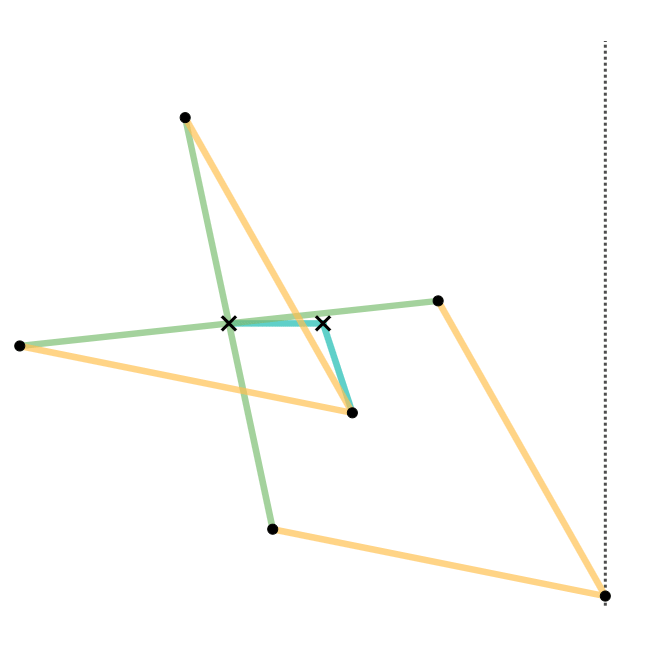
\includegraphics[width=\textwidth]{papers/geradlinig/figures/perrolatz_linkage3.png}
    \end{minipage}
    \caption{Der Mechanismus von Perrolatz~\cite{wiki_straight_line}.}
    \label{fig:perrolatz_link}
\end{figure}

Für diesen Mechanismus gelten die Beziehungen
$\overline{CO}=\overline{AO}=\overline{BO}=\overline{DO}$ sowie
$\overline{CE}=\overline{BE}=\overline{AF}=\overline{DF}$,
wie in Abbildung~\ref{fig:geometrie_perrolatz} dargestellt.
Der Punkt $E$ bewegt sich auf einer Kreisbahn, während der Punkt $O$ fest bleibt.
Dadurch bewegt sich der Punkt $F$ entlang einer Geraden.
Wie beim Peaucellier-Lipkin-Mechanismus muss auch hier die Kreisbahn 
durch den Punkt $O$ verlaufen.
Zusätzlich bleiben die Punkte $O$, $E$ und $F$ während der gesamten Bewegung kollinear.
\begin{figure}
    \centering
    \begin{tikzpicture}[scale=1.2]

  % Foints on/around circle
  \def\len{2}
  \coordinate (A) at ({\len*cos(60)},{\len*sin(60)});
  \coordinate (C) at ({\len*-cos(60)},{\len*sin(60)});
  \coordinate (B) at ({\len*-cos(60)},{\len*-sin(60)});
  \coordinate (D) at ({\len*cos(60)},{\len*-sin(60)});
  
  % Vertical line
  \def\r{1}
  \coordinate (O) at (0,0);
  \coordinate (P) at (0,{\len*sin(60)});
  \coordinate (E) at ({2*\r},0);
  \coordinate (F) at ({2*\r+2*\len*cos(60)},0);
  \draw[blue, thick] ({2*\r+2*\len*cos(60)},-2) -- ({2*\r+2*\len*cos(60)},2);
 
  % Circle 
  \draw[red, thick] (\r, 0) circle (\r);

  % Connections
  \draw[thick] (A) -- (O) -- (B) -- (E) -- (C);
  \draw[thick] (C) -- (D) -- (F) -- (A);

  % Additional green lines
  \draw[darkgreen, thin, dashed] (O) -- (E) node[midway, above] {$y$};
  \draw[darkgreen, thin, dashed] (O) -- (P) node[midway, left] {$h$};
  \draw[darkgreen, thin, dashed] (P) -- (C) node[midway, above] {$x$};
  \draw[darkgreen, thin, dashed] (P) -- (A) node[midway, above] {$x$};

  % Mark points
  \fill[black] (A) circle (1.5pt) node[above] {$A$};
  \fill[black] (B) circle (1.5pt) node[below] {$B$};
  \fill[black] (C) circle (1.5pt) node[above] {$C$};
  \fill[black] (D) circle (1.5pt) node[below] {$D$};
  \fill[black] (F) circle (1.5pt) node[right] {$F$};
  \fill[black] (E) circle (1.5pt) node[right] {$E$};
  \fill[black] (O) circle (1.5pt) node[left] {$O$};
  \fill[darkgreen] (P) circle (1.5pt) node[above] {$P$};

\end{tikzpicture}

    \caption{Kreisspiegelung am Perrolatz-Mechanismus.}
    \label{fig:geometrie_perrolatz}
\end{figure}
\begin{satz}
    Der Perrolatz-Mechanismus hat die Eigenschaft
    \begin{align}
        \overline{OE}\cdot\overline{OF} = R^2
        \label{eq:constant2}
    \end{align}
    einer Kreisspiegelung.
\end{satz}
\begin{proof} 
    Diese Bedingung lässt sich analog zum 
    Peaucellier-Lipkin-Mechanismus herleiten.
    Dazu definieren wir $\overline{CP}=\overline{PA}=x$, $\overline{CA}=\overline{EF}=2x$,
    $\overline{OP}=h$ und $\overline{OE}=y$,
    wobei $P$ die Mitte der Strecke $CA$ ist.
    Da $\overline{EF}=2x$ gilt, folgt $\overline{OF}=y+2x$.
    Damit kann man die Gleichung~\eqref{eq:constant2} schreiben als
    \begin{align*}
        \overline{OE}\cdot\overline{OF}
        =
        y(y+2x)
        =
        y^2+2xy.
    \end{align*}
    Mit dem Satz des Pythagoras erhält man
    \begin{align}
        \overline{CO}^2
        =
        x^2+h^2,
        \label{eq:CO}
    \end{align}
    sowie
    \begin{align}
        \overline{CE}^2
        =
        (y+x)^2+h^2
        =
        y^2+2xy+x^2+h^2.
        \label{eq:CE}
    \end{align}
    Subtrahiert man Gleichung~\eqref{eq:CO} von Gleichung~\eqref{eq:CE}, 
    erhält man
    \begin{align*}
        \overline{CE}^2-\overline{CO}^2
        =
        y^2+2xy
        =
        \overline{OE}\cdot\overline{OF}.
    \end{align*}
    Da die Längen $\overline{CE}$ und $\overline{CO}$ konstant sind, 
    ist das Produkt $\overline{OE}\cdot\overline{OF}$ konstant.
    Auch hier stellt sich heraus, dass die Konstante jeweils $R^2$ ist und
    bestätigt somit den Fall einer Kreisspiegelung.
\end{proof}